\documentclass{article}
\usepackage{comment}
\usepackage{amsmath}
\usepackage{amsfonts}
\usepackage{sectsty}
\usepackage{hyperref}
\usepackage{fancyhdr}
\usepackage[top=1in,bottom=1in,left=1in,right=1in]{geometry}
\usepackage{float}
\usepackage{graphicx}
\usepackage{tabularx}
\usepackage{mathtools}

\title{Assignment 2}
\author{Matthew Farah, \href{mailto:farahm11@mcmaster.ca}{$\langle$farahm11@mcmaster.ca$\rangle$}, 400468251}
\date{\today}

\hypersetup{
        colorlinks=true,
        linkcolor=blue,
        filecolor=magenta,
        urlcolor=blue,
        citecolor=blue,
	anchorcolor=blue
}

\fancyhead{}
\fancyhead[L]{Matthew Farah, \href{mailto:farahm11@mcmaster.ca}{$\langle$farahm11@mcmaster.ca$\rangle$}, 400468251}
\fancyhead[R]{Assignment 2}

\newenvironment{directsubsubs}{
  \makeatletter
  \renewcommand\thesubsubsection{\thesection.\Roman{subsubsection}}
  \makeatother
}{
  \makeatletter
  \renewcommand\thesubsubsection{\thesubsection.\Roman{subsubsection}}
  \makeatother
}

\renewcommand{\thesubsection}{\thesection.\alph{subsection}}
\renewcommand{\thesubsubsection}{\thesection.\alph{subsection}.\Roman{subsubsection}}
\makeatletter
\DeclareFontFamily{U}{MnSymbolA}{}
\DeclareFontShape{U}{MnSymbolA}{m}{n}{
    <-6>  MnSymbolA5
   <6-7>  MnSymbolA6
   <7-8>  MnSymbolA7
   <8-9>  MnSymbolA8
   <9-10> MnSymbolA9
  <10-12> MnSymbolA10
  <12->   MnSymbolA12}{}
\DeclareFontShape{U}{MnSymbolA}{b}{n}{
    <-6>  MnSymbolA-Bold5
   <6-7>  MnSymbolA-Bold6
   <7-8>  MnSymbolA-Bold7
<8-9>  MnSymbolA-Bold8
   <9-10> MnSymbolA-Bold9
  <10-12> MnSymbolA-Bold10
  <12->   MnSymbolA-Bold12}{}
\DeclareSymbolFont{MnSyA}{U}{MnSymbolA}{m}{n}
\SetSymbolFont{MnSyA}{bold}{U}{MnSymbolA}{b}{n}

\DeclareRobustCommand{\overleftharpoon}{\mathpalette{\overarrow@\leftharpoonfill@}}
\DeclareRobustCommand{\overrightharpoon}{\mathpalette{\overarrow@\rightharpoonfill@}}
\def\leftharpoonfill@{\arrowfill@\leftharpoondown\mn@relbar\mn@relbar}
\def\rightharpoonfill@{\arrowfill@\mn@relbar\mn@relbar\rightharpoonup}

\DeclareMathSymbol{\leftharpoondown}{\mathrel}{MnSyA}{'112}
\DeclareMathSymbol{\rightharpoonup}{\mathrel}{MnSyA}{'100}
\DeclareMathSymbol{\mn@relbar}{\mathrel}{MnSyA}{'320}
\makeatother


\newcolumntype{Y}{>{\centering\arraybackslash}X}
\renewcommand{\arraystretch}{1.8}

\sectionfont{\fontsize{12}{12}\bfseries}
\subsectionfont{\fontsize{10}{12}\normalfont}
\subsubsectionfont{\fontsize{10}{12}\normalfont}

\newcommand{\harpoon}[1]{\overrightharpoonup{#1}}

\begin{document}
\maketitle
\pagestyle{fancy}

\begin{center}
	\Large{\underline{Impulse Response}}
\end{center}
\section[Question ~\thesection]{Given the system $y(n) - y(n - 1) - y(n - 2) + x(n)$:}

\subsection[~\thesubsection]{Determine the $(A, B , C, D)$ representation of the system.}

\subsubsection[~\thesubsubsection]{Find $\overrightharpoon{S(n)}$}

\begin{align*}
	&\text{Let:}& \text{Then:} \\
	&s_1(n) = y(n - 2) &s_1(n + 1) = y(n - 1) = s_2(n) \\
	&s_2(n) = y(n - 1) &s_2(n + 1) = \\
	& &= y(n) \\
	& &= -y(n - 2) + y(n - 1) + x(n) \\
	& &=-s_1(n) + s_2(n) + x(n)
\end{align*}

Thus, let $\overrightharpoon{S(n)} = \begin{psmallmatrix} s_1(n) \\ s_2(n)\end{psmallmatrix}$

\subsubsection[~\thesubsubsection]{Find $\overrightharpoon{S(n + 1)}$}

\begin{align*}
	\overrightharpoon{S(n + 1)} &= \begin{pmatrix} s_1(n + 1) \\ s_2(n + 1) \end{pmatrix} \\
	&= \begin{pmatrix} s_2(n) \\ -s_1(n) + s_2(n) + x(n) \end{pmatrix} \\
	&= \begin{pmatrix} 0 & 1 \\ -1 & 1 \end{pmatrix}\overrightharpoon{S(n)} + \begin{pmatrix} 0 \\ 1\end{pmatrix}x(n)
\end{align*}

Therefore, our $\boldsymbol{A}$ and $\boldsymbol{B}$ matrices are $\begin{psmallmatrix} 0 & 1 \\ -1 & 1 \end{psmallmatrix}$ and $\begin{psmallmatrix} 0 \\ 1 \end{psmallmatrix}$ respectively.

\subsubsection[~\thesubsubsection]{Find $y(n)$}

\begin{align*}
	y(n) &= -y(n - 2) + y(n - 1) + x(n) \\
	&= -s_1(n) + s_2(n) + x(n) \\
	&= \begin{pmatrix} -1 & 1 \end{pmatrix}\overrightharpoon{S(n)} + \begin{pmatrix} 1 \end{pmatrix}x(n)
\end{align*}

Therefore, our $\boldsymbol{C}$ and $\boldsymbol{D}$ matrices are $\begin{psmallmatrix} -1 & 1 \end{psmallmatrix}$ and $\begin{psmallmatrix} 1 \end{psmallmatrix}$ respectively.

Putting it all together, our system can be represented in state space form as:

\begin{align*}
	\overrightharpoon{S(n + 1)} &= \begin{pmatrix} 0 & 1 \\ -1 & 1 \end{pmatrix}\overrightharpoon{S(n)} + \begin{pmatrix} 0 \\ 1\end{pmatrix} \\\\
	y(n) &= \begin{pmatrix} -1 & 1\end{pmatrix}\overrightharpoon{S(n)} + \begin{pmatrix} 1 \end{pmatrix}x(n)
\end{align*}

\subsection{Compute the impulse response $h(n)$}

To compute the impulse response, we will use the state space-equations and solve for the input $x(n) = \delta(n)$.

\begin{align*}
	&\underline{\text{Current State} \; (\overrightharpoon{S(n)})}& &\underline{\text{Current Output} \; (y(n))} \\ \\
	&\overrightharpoon{S(0)} = \overrightharpoon{0}& &y(0) = \begin{pmatrix} -1 & 1 \end{pmatrix}\overrightharpoon{S(0)} + \begin{pmatrix} 1 \end{pmatrix}x(0) = 1 \\
	&\overrightharpoon{S(1)} = \begin{pmatrix} 0 & 1 \\ -1 & 1 \end{pmatrix}\overrightharpoon{S(0)} + \begin{pmatrix} 0 \\ 1 \end{pmatrix}x(0) = \begin{pmatrix} 0 \\ 1 \end{pmatrix}& &y(1) = \begin{pmatrix} -1 & 1 \end{pmatrix}\overrightharpoon{S(1)} + \begin{pmatrix} 1 \end{pmatrix}x(1) = 1 \\
	&\overrightharpoon{S(2)} = \begin{pmatrix} 0 & 1 \\ -1 & 1 \end{pmatrix}\overrightharpoon{S(1)} + \begin{pmatrix} 0 \\ 1 \end{pmatrix}x(1) = \begin{pmatrix} 1 \\ 1 \end{pmatrix}& &y(2) = \begin{pmatrix} -1 & 1 \end{pmatrix}\overrightharpoon{S(2)} + \begin{pmatrix} 1 \end{pmatrix}x(2) = 0 \\
	&\overrightharpoon{S(3)} = \begin{pmatrix} 0 & 1 \\ -1 & 1 \end{pmatrix}\overrightharpoon{S(2)} + \begin{pmatrix} 0 \\ 1 \end{pmatrix}x(2) = \begin{pmatrix} 1 \\ 1 \end{pmatrix}& &y(3) = \begin{pmatrix} -1 & 1 \end{pmatrix}\overrightharpoon{S(3)} + \begin{pmatrix} 1 \end{pmatrix}x(3) = 0 \\
	&\overrightharpoon{S(4)} = \begin{pmatrix} 0 & 1 \\ -1 & 1 \end{pmatrix}\overrightharpoon{S(3)} + \begin{pmatrix} 0 \\ 1 \end{pmatrix}x(3) = \begin{pmatrix} 1 \\ 1 \end{pmatrix}& &y(4) = \begin{pmatrix} -1 & 1 \end{pmatrix}\overrightharpoon{S(4)} + \begin{pmatrix} 1 \end{pmatrix}x(4) = 0 \\
	&\vdots& &\vdots
\end{align*}

Therefore, the impulse response of the system is given by $h(n) = \begin{cases}1, \; \text{if} \; n = 0, 1 \\ 0, \; \text{otherwise} \end{cases} = \delta(n) + \delta(n - 1)$.

\newpage

\begin{center}
	\Large{\underline{Convolutional Systems}}
\end{center}

\section[Question ~\thesection]{An LTI system is described by the impulse response $h(n) = \delta(n) + \delta(n - 2)$. Determine the output of the system for the input $\delta(n) + \delta(n - 2) + \delta(n - 4)$.}

We can do this in 1 of two ways

\begin{directsubsubs}

	\subsubsection{Solve using the LTI properties of the system}
	Since we know $h(n) = \delta(n) + \delta(n - 2)$, that implies that to output of the system $y(n) = \delta(n) + \delta(n - 2)$ when $x(n) = \delta(n)$. Therefore. Since the system is LTI (linear, time-invariant), we can deduce that:

	\begin{align*}
		y(n) &= h(n) + h(n - 2) + h(n - 4) \\
		&= \delta(n) + \delta(n - 2) + \delta(n - 2) + \delta(n - 4) + \delta(n - 4) + \delta(n - 6) \\
		&= \delta(n) + 2\delta(n - 2) + 2\delta(n - 4) + \delta(n - 6)
	\end{align*}

	Thus, the output of the system is given by $y(n) = \begin{cases} 1 \; \text{if} \; n = 0, 6 \\ 2, \; \text{if} \; n = 2, 4 \\0, \; \text{otherwise} \end{cases} = \delta(n) + 2\delta(n - 2) + 2\delta(n - 4) + \delta(n - 6)$.

	\subsubsection{Solve using the convolutional equation}
	Using the convolutional equation, we can determine that:

	\begin{align*}
		y(n) &= \sum_{k = -\infty}^{\infty} (h(n - k)x(k)) \\[4pt]
		&= \sum_{k = -\infty}^{\infty} 
			\Bigl( (\delta(n - k) + \delta(n - k - 2))
			 (\delta(k) + \delta(k - 2) + \delta(k - 4)) \Bigr) \\[4pt]
		&= \sum_{k = -\infty}^{\infty} 
		\begin{aligned}[t]
			(&\delta(n - k)\delta(k) 
			+ \delta(n - k)\delta(k - 2) 
			+ \delta(n - k)\delta(k - 4) \\
			&+ \delta(n - k - 2)\delta(k)
			+ \delta(n - k - 2)\delta(k - 2)
			+ \delta(n - k - 2)\delta(k - 4))
		\end{aligned} \\[4pt]
		&= \delta(0)\delta(n) + \delta(0)\delta(n - 2) + \delta(0)\delta(n - 4)
		   + \delta(0)\delta(n - 2) + \delta(0)\delta(n - 4) + \delta(0)\delta(n - 6) \\[4pt]
		&= \delta(n) + \delta(n - 2) + \delta(n - 4) 
		   + \delta(n - 2) + \delta(n - 4) + \delta(n - 6) \\[4pt]
		&= \delta(n) + 2\delta(n - 2) + 2\delta(n - 4) + \delta(n - 6)
	\end{align*}

	Thus, the output of the system is given by $y(n) = \begin{cases} 1 \; \text{if} \; n = 0, 6 \\ 2, \; \text{if} \; n = 2, 4 \\0, \; \text{otherwise} \end{cases} = \delta(n) + 2\delta(n - 2) + 2\delta(n - 4) + \delta(n - 6)$.

\end{directsubsubs}

\newpage

\begin{center}
	\Large{\underline{Convolution}}
\end{center}

\section[Question ~\thesection]{Given the impulse response $h(n) = \begin{cases} 1, \; \text{if} \; n = 0 \\2,  \; \text{if} \; n = 1 \\3, \; \text{if} \; n = 2\\0 \; \text{otherwise} \end{cases}$, determine:}

\subsection[~\thesubsection]{The difference equation for the system}

We know that when $x(n) = \delta(n)$, $y(n) = \begin{cases} 1, \; \text{if} \; n = 0 \\2,  \; \text{if} \; n = 1 \\3, \; \text{if} \; n = 2\\0 \; \text{otherwise} \end{cases}$. Therefore, we know:

\begin{align*}
	y(n) &= \delta(n) + 2\delta(n - 1) + 3\delta(n - 2)
\end{align*}

Substituting in, using the fact $\delta(n) = x(n)$, we have:

\begin{align*}
	y(n) &= x(n) + 2x(n - 1) + 3x(n - 2)
\end{align*}

Giving us the difference equation of our system.

\subsection[~\thesubsection]{The $(A, B, C, D)$ representation of the system}

\subsubsection[~\thesubsubsection]{Find $\overrightharpoon{S(n)}$}

To do this, we will use the difference equation for the system derives in a.).

\begin{align*}
	&\text{Let:}& \text{Then:} \\
	&s_1(n) = x(n - 2)& &s_1(n + 1) = x(n - 1) = s_2(n) \\
	&s_2(n) = x(n - 1)& &s_2(n + 1) = x(n)
\end{align*}

Thus, let $\overrightharpoon{S(n)} = \begin{psmallmatrix} s_1(n) \\ s_2(n) \end{psmallmatrix}$

\subsubsection[~\thesubsubsection]{Find $\overrightharpoon{S(n + 1)}$}

\begin{align*}
	\overrightharpoon{S(n + 1)} &= \begin{pmatrix} s_1(n + 1) \\ s_2(n + 1) \end{pmatrix} \\
	&= \begin{pmatrix} s_2(n) \\ x(n) \end{pmatrix} \\
	&= \begin{pmatrix} 0 & 1 \\ 0 & 0 \end{pmatrix}\overrightharpoon{S(n)} + \begin{pmatrix} 0 \\ 1 \end{pmatrix}x(n)
\end{align*}

Therefore, our $\boldsymbol{A}$ and $\boldsymbol{B}$ matrices are $\begin{psmallmatrix} 0 & 1 \\ 0 & 0 \end{psmallmatrix}$ and $\begin{psmallmatrix} 0 \\ 1 \end{psmallmatrix}$ respectively.

\subsubsection[~\thesubsubsection]{Find $y(n)$}

\begin{align*}
	y(n) &= 3x(n - 2) + 2x(n - 1) + x(n) \\
	&= 3s_1(n - 2) + 2s_2(n - 1) + x(n) \\
	&= \begin{pmatrix} 3 & 2 \end{pmatrix}\overrightharpoon{S(n)} + \begin{pmatrix} 1 \end{pmatrix}x(n)
\end{align*}

Therefore, our $\boldsymbol{C}$ and $\boldsymbol{D}$ matrices are $\begin{psmallmatrix} 3 & 2 \end{psmallmatrix}$ and $\begin{psmallmatrix} 1 \end{psmallmatrix}$ respectively.

Putting it all together, our system can be represented in state space form as:

\begin{align*}
	\overrightharpoon{S(n + 1)} &= \begin{pmatrix} 0 & 1 \\ 0 & 0 \end{pmatrix}\overrightharpoon{S(n)} + \begin{pmatrix} 0 \\ 1 \end{pmatrix}x(n) \\\\
	y(n) &= \begin{pmatrix} 0 & 1 \\ 0 & 0 \end{pmatrix}\overrightharpoon{S(n)} + \begin{pmatrix} 0 \\ 1 \end{pmatrix}x(n)
\end{align*}

\subsection[~\thesubsection]{The outputs of the system using convolutions for the input $x(n) = \delta(n) + \delta(n - 1) + \delta(n - 3)$}

Using the convolutional equation, we can compute that the output of this system for the input $x(n) = \delta(n) + \delta(n - 1) + \delta(n - 3)$ is given by:

\begin{align*}
	y(n) &= \sum_{k = -\infty}^{\infty}(h(n - k)x(k)) \\
	&= \sum_{k = -\infty}^{\infty}(h(n - k)(\delta(k) + \delta(k - 1) + \delta(k - 3))) \\
	&= \sum_{k = -\infty}^{\infty}(h(n - k)\delta(k) + h(n - k)\delta(k - 1) + h(n - k)\delta(k - 3)) \\
	&= h(n) + h(n - 1) + h(n - 3)
\end{align*}

And since we know $h(n) = \begin{cases} 1, \; \text{if} \; n = 0 \\2,  \; \text{if} \; n = 1 \\3, \; \text{if} \; n = 2\\0 \; \text{otherwise} \end{cases} = \delta(n) + 2\delta(n - 1) + 3\delta(n - 2)$, can conclude that:

\begin{align*}
	y(n) &= h(n) + h(n - 1) + h(n - 3) \\
	&= \delta(n) + 2\delta(n - 1) + 3\delta(n - 2) + \delta(n - 1) + 2\delta(n - 2) + 3\delta(n - 3) + \delta(n - 3) + 2\delta(n - 4) + 3\delta(n - 5) \\
	&= \delta(n) + 3\delta(n - 1) + 5\delta(n - 2) + 4\delta(n - 3) + 2\delta(n - 4) + 3\delta(n - 5)
\end{align*}

Therefore, the system's outputs for the input $x(n) = \delta(n) + \delta(n - 1) + \delta(n - 3)$ is given by:
\begin{align*}
	y(n) &= \begin{cases} 1, \; \text{if} \; n = 0 \\3, \; \text{if} \; n = 1 \\5, \; \text{if} \; n = 2 \\4, \; \text{if} \; n = 3 \\2, \; \text{if} \; n = 4 \\3, \; \text{if} \; n = 5 \\0, \; \text{otherwise} \end{cases} \\\\
	&= \delta(n) + 3\delta(n - 1) + 5\delta(n - 2) + 4\delta(n - 3) + 2\delta(n - 4) + 3\delta(n - 5)
\end{align*}

Note here as well that we could have arrived at the conclusion that $y(n) = h(n) + h(n - 1) + h(n - 3)$ for the input $x(n) = \delta(n) + \delta(n - 1) + \delta(n - 3)$ without the use of the convolutional equation since, from a.), we know the system has no feedback and thus must be FIR.

\newpage

\begin{center}
	\Large{\underline{Complex Numbers}}
\end{center}

\section[Question ~\thesection]{Solve the following questions pertaining to complex numbers:}

\subsection[~\thesubsection]{Convert $-1 - i$ into exponential form}

%FIX:!!!!!

\begin{figure}[H]
	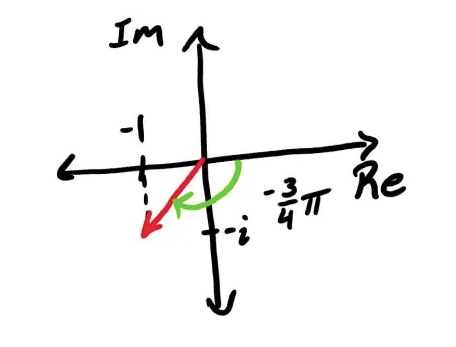
\includegraphics[width=\linewidth]{./imgs/Question-4-a.png}
	\caption{$-1 - i$ in the complex plane.}
\end{figure}

\begin{align*}
	|-1 - i| &= \sqrt{((-1)^2 + (-1)^2)} = \sqrt{2} \\
	arg(-1 - i) &= \frac{-3\pi}{4}
\end{align*}

Therefore, $-1 - i = \sqrt{2}e^{-\frac{3\pi}{4}i}$

\subsection[~\thesubsection]{Compute $|e^{i{\frac{\pi}{2}}}|$}

By the definition of complex exponentials, $|e^{\frac{\pi}{2}i}| = 1$.

\subsection[~\thesubsection]{Convert $-2$ into exponential form}

\begin{figure}[H]
	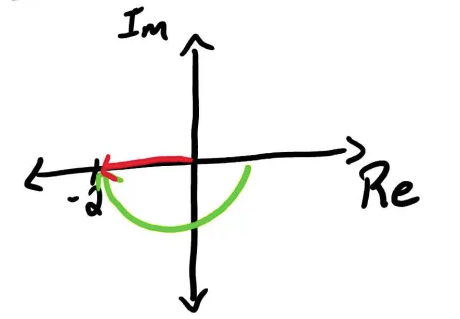
\includegraphics[width=\linewidth]{./imgs/Question-4-c.png}
	\caption{$-2$ in the complex plane.}
\end{figure}

\begin{align*}
	|-2| &= 2 \\
	arg(-2) &= -\pi
\end{align*}

Therefore, $-2 = e^{{-\pi}i}$.

\subsection[~\thesubsection]{Find $arg(1 - i)$}

\begin{figure}[H]
	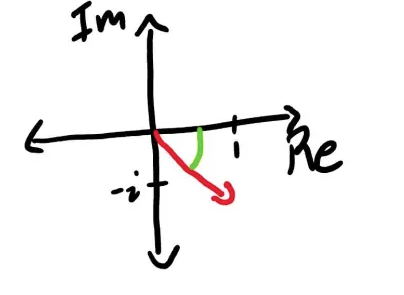
\includegraphics[width=\linewidth]{./imgs/Question-4-d.png}
	\caption{$1 - i$ in the complex plane.}
\end{figure}

Therefore, $arg(1 - i) = \frac{-\pi}{4} \pm 2{\pi}k \qquad k \; \in \; \mathbb{Z}$.

\subsection[~\thesubsection]{Convert $-i$ into exponential form}

\begin{figure}[H]
	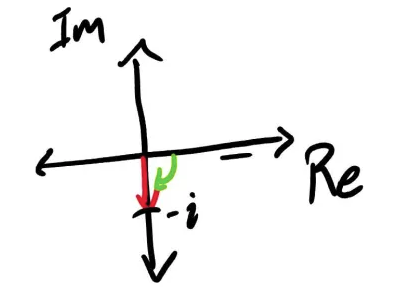
\includegraphics[width=\linewidth]{./imgs/Question-4-e.png}
	\caption{$-i$ in the complex plane.}
\end{figure}

\begin{align*}
	|-i| &= \sqrt{(-1)^2} = \sqrt{1} = 1 \\
	arg(-i) &= \frac{-\pi}{2}
\end{align*}

Therefore, $-i = e^{-\frac{\pi}{2}i}$.

\end{document}
